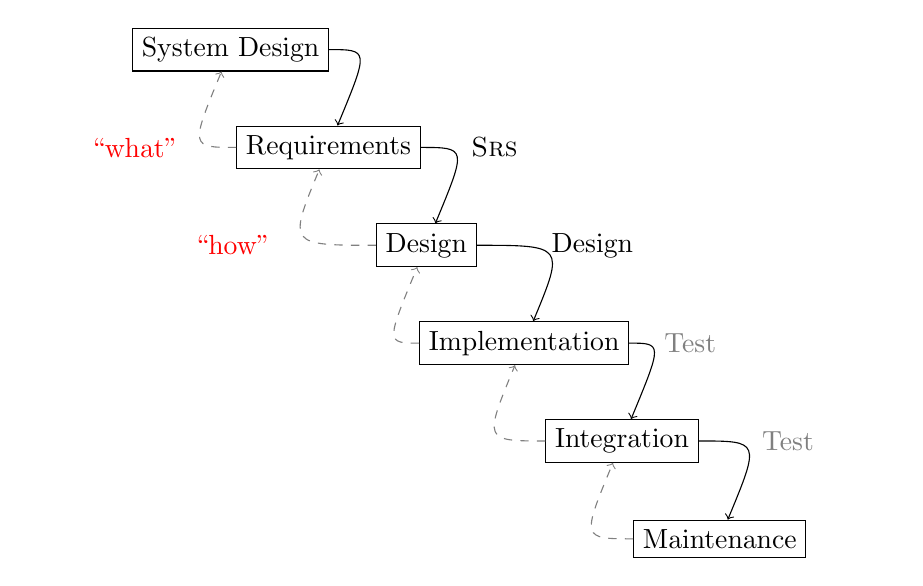
\begin{tikzpicture}[node distance=50]

\node[draw] (1) at (0,0) {System Design};
\node[draw] (2) [below right of = 1] {Requirements};
\node[draw] (3) [below right of = 2] {Design};
\node[draw] (4) [below right of = 3] {Implementation};
\node[draw] (5) [below right of = 4] {Integration};
\node[draw] (6) [below right of = 5] {Maintenance};

\node (c1) [right of = 1] {};
\node (c2) [right of = 2] {};
\node (c3) [right of = 3] {};
\node (c4) [right of = 4] {};
\node (c5) [right of = 5] {};
\node (c6) [right of = 6] {};

\node (1c) [left of = 1] {};
\node (2c) [left of = 2] {};
\node (3c) [left of = 3] {};
\node (4c) [left of = 4] {};
\node (5c) [left of = 5] {};
\node (6c) [left of = 6] {};

\path[draw,->] (1) .. controls (c1) .. (2);
\path[draw,->] (2) .. controls (c2) .. (3);
\path[draw,->] (3) .. controls (c3) .. (4);
\path[draw,->] (4) .. controls (c4) .. (5);
\path[draw,->] (5) .. controls (c5) .. (6);

\node[node distance=10] (a1) [right of = c1] {};
\node[node distance=10] (a2) [right of = c2] {\textsc{Srs}};
\node[node distance=10] (a3) [right of = c3] {Design};
\node[node distance=10] (a4) [right of = c4] {\textcolor{gray}{Test}};
\node[node distance=10] (a5) [right of = c5] {\textcolor{gray}{Test}};
\node[node distance=10] (a6) [right of = c6] {};

\path[draw,dashed,color=gray,->] (2) .. controls (2c) .. (1);
\path[draw,dashed,color=gray,->] (3) .. controls (3c) .. (2);
\path[draw,dashed,color=gray,->] (4) .. controls (4c) .. (3);
\path[draw,dashed,color=gray,->] (5) .. controls (5c) .. (4);
\path[draw,dashed,color=gray,->] (6) .. controls (6c) .. (5);

\node[node distance=20] (1a) [left of = 1c] {};
\node[node distance=20] (2a) [left of = 2c] {\textcolor{red}{``what''}};
\node[node distance=20] (3a) [left of = 3c] {\textcolor{red}{``how''}};
\node[node distance=20] (4a) [left of = 4c] {};
\node[node distance=20] (5a) [left of = 5c] {};
\node[node distance=20] (6a) [left of = 6c] {};

\end{tikzpicture}